Wir haben mithilfe von UML-Diagrammen die konzeptionelle Sicht realisiert. Im Folgenden werden die einzelnen Diagramme aufgezeigt und beschrieben und in nachfolgenden Sichten zusätzlich verfeinert und konkretisiert.

\subsection{Überblick}
\label{Ueberblick}

\begin{figure} [H] 
\caption{Konzeptionelle Sicht (Klein)} \centering
	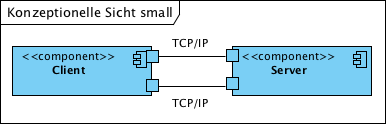
\includegraphics[scale=2]{Diagramme/KonzeptionelleSichtKlein.png} 
	\label{pic:konzeptionellesichtklein} 
\end{figure}

Unsere Architektur besteht aus zwei grundlegenden Komponenten, der Serverkomponente und der Clientkomponente (siehe Abb. \vref{pic:konzeptionellesichtklein} und Abb. \vref{pic:konzeptionellesicht}). Diese Komponenten beinhalten wiederum weitere Komponenten. Auf der einen Seite haben wir unsere Serverkomponente, die alle benötigten Daten für die Quizfragen, der Nutzer sowie z.B. Punkteständen usw. der App speichert.

Auf der anderen Seite, der Clientkomponente, muss zwischen zwei Komponenten unterschieden werden. Einmal der Komponente GUI-Client, welche sich in erster Linie an den Administrator, der über eine Webseite die Spiele konfigurieren und die Fragen und Antworten redaktionell bearbeiten kann, richtet und dann noch der mobile Android-Client, der sich ausschließlich an die Nutzer bzw. Spieler richtet.

Der GUI-Client stellt für die Verantwortlichen bzw. die Administratoren alle benötigten Funktionen bereit, um die App zu verwalten. Der Android-Client ermöglicht dem Spieler, die Quizapp zu spielen und Einstellungen vorzunehmen. 

\begin{figure} [H] 
\caption{Konzeptionelle Sicht}  \centering
	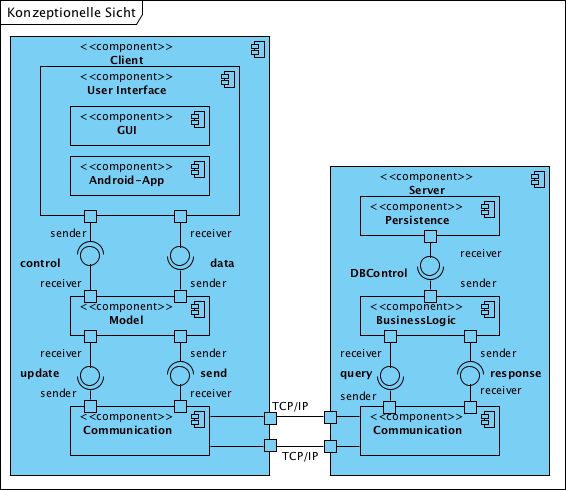
\includegraphics[width=1\textwidth]{Diagramme/KonzeptionelleSicht.png} 
	\label{pic:konzeptionellesicht} 
\end{figure}

{\centering Als Architekturstil verwenden wir das Model-View-Controller-Pattern.\\}

\subsection{Serverkomponente}
\label{sec:server}

\begin{figure} [H] 
\caption{Konzeptionelle Sicht Server}  \centering
	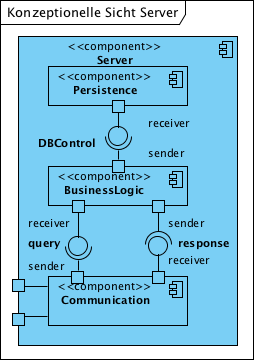
\includegraphics[scale=1.85]{Diagramme/KonzeptionelleSichtServer.png} 
	\label{pic:konzeptionellesichtserver} 
\end{figure}

Die Serverkomponente (siehe Abb. \vref{pic:konzeptionellesichtserver} besteht aus insgesamt drei Teilkomponenten, welche sich wie folgt aufgliedern:

\begin{itemize}
\item{Communication}

Die Komponente \texttt{Communication} nimmt Anfragen des Clients entgegen und leitet sie an die Komponente \texttt{BusinessLogic} weiter, wo die Anfragen verarbeitet werden und sendet die Ergebnisse zurück an den Client.

\item{BusinessLogic}

Die Komponente \texttt{BusinessLogic} dient zum Verarbeiten der Anfragen und leitet diese verarbeiteten Anfragen dann an die Komponente \texttt{Persistence} weiter.

\item{Persistence}

Die Komponente \texttt{Persistence} ist die Schnittstelle zur Datenbank. Über das Interface \texttt{DBControl} werden die verarbeiteten Anfragen von der Komponente \texttt{BusinessLogic} empfangen und in Datenbankabfragen umgewandelt, welche dann von der Datenbank entgegen genommen werden.

\end{itemize}

\subsection{Clientkomponente}
\label{sec:client}

\begin{figure} [H] 
\caption{Konzeptionelle Sicht Client}  \centering
	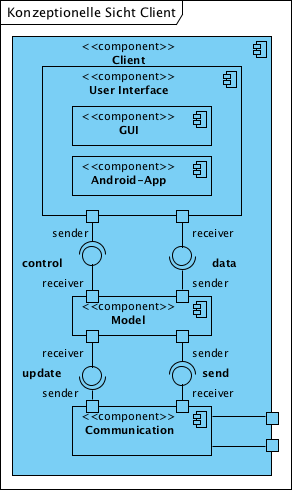
\includegraphics[scale=2]{Diagramme/KonzeptionelleSichtClient.png} 
	\label{pic:konzeptionellesichtclient} 
\end{figure}

Die Clientkomponente (siehe Abb. \vref{pic:konzeptionellesichtclient} besteht so wie die Serverkomponente aus drei Teilkomponenten, welche sich wie folgt aufgliedern:

\begin{itemize}
\item{Communication}

Die Komponente \texttt{Communication} sendet Anfragen des Clients an den Server, welche dort verarbeitet werden und nimmt die Ergebnisse entgegen, um diese an die Komponente \texttt{Model} zu übergeben, wo die Ergebnisse der Anfrage weiter verarbeitet werden.

\item{Model}

Die Komponente \texttt{Model} nimmt Ergebnisse von der Komponente \texttt{Communication} entgegen und schickt diese an die Komponente \texttt{User Interface}. 

\item{User Interface}

Die Komponente \texttt{User Interface} muss in zwei unterschiedliche Komponenten zerlegt werden:
\begin{itemize}
\item{GUI}

Die GUI richtet sich in erster Linie an den Administrator bzw. die Verantwortlichen und nimmt alle möglichen Aktionen des Administrators entgegen und schickt diese an die Komponente \texttt{Model}, um weiter verarbeitet zu werden. Sie bildet ebenfalls eine eigenständige Komponente.

\item{Android-App}

Die Android-App richtet sich ausschließlich an die Nutzer bzw. Spieler der App und bietet ihnen die Funktionen, die in der Anforderungsspezifikation erarbeitet wurden. Zu diesen gehören z.B. das Registrieren beim Server sowie das Spielen von Fragerunden oder das Anzeigenlassen von Ranglisten oder sonstigen spielerelevanten Statistiken.

\end{itemize}

\end{itemize}